\documentclass[floatfix]{article}  
\pagestyle{plain}

\usepackage{amsmath,amssymb}
\usepackage{dsfont}
\usepackage{graphicx} %loads the graphicx.sty package 
\usepackage{epstopdf} %loads the epstopdf.sty package {slashed}
\usepackage{color}

\usepackage{graphicx,longtable,tocloft,color}
\usepackage{sidecap}
\usepackage{subfig}
\usepackage{xspace}
\usepackage{mydefs}
\usepackage{cite}
\usepackage{lineno}
\usepackage{multirow}
\usepackage{hyperref}
\usepackage[left=2.8cm,right=2.8cm,top=2.5cm,bottom=3.5cm]{geometry}
\usepackage{caption}
%\tolerance = 1000
%\parindent 0cm
%\parskip 2mm
%
%
%for draft only:
%\linenumbers
\usepackage{array}


\title{Constraining new physics with collider measurements of Standard Model signatures}

\author{Jonathan M. Butterworth$^1$, David Grellscheid$^2$,\\[1mm] Michael Kr\"amer$^3$, David Yallup$^1$\\[2.5mm]
\it $^1$Department of Physics and Astronomy, University College London,\\ \it Gower St., London, WC1E 6BT, UK\\[1mm]
\it $^2$IPPP, Department of Physics,\\\it Durham University, DH1 3LE, UK\\[1mm] \it $^3$Institute for Theoretical Particle Physics and Cosmology, \\ \it RWTH Aachen University, D-52056 Aachen, Germany}


\begin{document}

\maketitle 

\begin{abstract}
A new method providing general consistency contraints for Beyond-the-Standard-Model (BSM) theories, using 
measurements at particle colliders, is presented. The method, `Constraints On New Theories Using \rivet' - \Contur \ - exploits
the fact that particle-level differential measurements made in fiducial regions of phase-space have a high degree of
model-independence. These measurements can therefore be compared to BSM physics implemented in Monte Carlo generators in a very
generic way, allowing a wider array of final states to be considered than is typically the case. The \Contur approach should be seen
as complementary to the discovery potential of direct searches, being designed to eliminate inconsistent 
BSM proposals in a context where many (but perhaps not all) measurements are consistent with the Standard Model.
We demonstrate, using a competitive simplified dark matter model, the power of this approach. 
The \Contur method is highly scaleable to other models and future measurements.
%
\begin{flushright}IPPP/16/52, MCNET-16-nn, TTK-16-nn\end{flushright}
\end{abstract}


\section{Introduction}
\label{sec:intro}
\todo{confirm MCnet preprint number on submission day at \url{http://montecarlonet.org/index.php?p=Publications/2016}}
The Large Hadron Collider (LHC) is probing physics in a new kinematic region, at energies around and above the 
electroweak symmetry-breaking scale. With the discovery of the Higgs boson~\cite{Aad:2012tfa,Chatrchyan:2012ufa}, 
the first data-taking period of the LHC experiments demonstrated that the understanding of electroweak symmetry-breaking within
the Standard Model (SM) is broadly correct, and thus that the theory is potentially valid well above the
TeV scale. Many precision measurements of jets, charged leptons, and other final states 
have been published, reaching into this new kinematic domain. The predictions of the SM are 
generally in agreement with the data, while the many dedicated searches for physics beyond the SM
have excluded a wide range of possible scenarios. 
%Nevertheless, there are many reasons to be confident that
%physics beyond the Standard Model (BSM) exists; examples include the gravitational evidence for dark matter, the large 
%preponderance of matter over antimatter in the universe, and the existence of gravity itself. None of 
%these can be easily accommodated within known Standard Model phenomenology. 
Nevertheless, there are many reasons to be confident that
physics beyond the Standard Model (BSM) exists, including in particular the gravitational evidence for dark matter, which cannot be accommodated within the 
Standard Model. \textbf{MK: have removed the reference to the matter-antimatter asymmetry and to gravity, as it is not really related to BSM at the TeV scale.} 


This motivates a continued campaign to make precise measurements and calculations at higher energies and 
luminosities, and to exploit these measurements to narrow down the class of viable models of new physics, 
hopefully shedding light on the correct new theory, or at least on the energy scale at which
new physics might be observed at future experiments. Whether physics beyond the Standard Model is discovered 
or not, there is a need to extract the clearest and most generic information about physics in this new energy regime,
an imperative which will grow with integrated luminosity. 

In this paper we exploit three important developments to survey existing measurements and set 
limits on new physics. 

\begin{enumerate}
\item
SM predictions for differential and exclusive, or semi-exclusive, final states are made using sophisticated 
calculational software, often embedded in Monte Carlo generators capable of simulating full, realistic final 
states~\cite{Buckley:2011ms}. These generators now incorporate matrix-elements for higher-order processes
matched to logarithmic parton showers, and successful models of soft physics such as hadronisation and
the underlying event. They are also capable of importing new physics models into this framework, thus allowing
the rapid prediction of their impact on a wide variety of final states simultaneously. 
In this paper we make extensive use of these capabilities within Herwig~\cite{Bahr:2008pv} \todo{DG: Herwig 7 cite}.\todo{MK: should we always use special fonts like small caps for computer tools (Herwig, Feynrules, rivet etc.)?}
\item
As the search for many of the favoured BSM scenarios has been unsuccessful, there has been a move toward 
``simplified models'' of new physics~\cite{Alves:2011wf,Abercrombie:2015wmb}, which aim to be as generic as possible 
and which provide a framework for interpreting BSM signatures with a minimal amount of 
new particles, interactions and model assumptions. The philosophy is similar to an ``effective lagrangian'' approach in which effective anomalous
couplings are introduced to describe new physics, but is more powerful, as such simplified models also
include new particles, and thus can remain useful up to and beyond the scale of new physics -- a region 
potentially probed by LHC measurements.
\item
The precision measurements from the LHC have mostly been made in a manner which minimises their model-dependence. 
That is, they are defined in terms of final-state signatures in fiducial regions well-matched to the
acceptance of the detector. Many such measurements are readily available for analysis and
comparison in the \rivet library~\cite{Buckley:2010ar}. 
\end{enumerate}

These three developments together make it possible to efficiently 
bring the power of a very wide range of data to bear on the search for new physics. While such a generic approach is
unlikely to compete in terms of speed and sensitivity with a search optimised for a specific theory, the breadth
of potential signatures and models which can be covered makes it a powerful complementary approach.\footnote{Limits from existing 
searches can sometimes be applied to new models, for example by accessing archived versions of the original analysis code
and detector simulation via the RECAST~\cite{Cranmer:2010hk} project.}
Any theory seeking
to explain a new signature or anomaly in the data may predict a BSM signal \todo{DG: clarify} in other final states, which should be checked 
against data this way. If, on the other hand, no BSM physics emerges, a model-independent and systematic approach becomes mandatory to exclude 
new physics models or narrow down the corresponding model parameter space.\todo{DG: clarify}

In this paper, we first motivate and describe the 
simplified model we have chosen as an initial demonstration, and its simulation using Feynrules~\cite{Alloul:2013bka} and Herwig~\cite{}. \textbf{[MK: added citation here because its the first mention of Feynrules. Maybe  better mention it before and drop citation here....]}
In Section~\ref{sec:measurements} we introduce the measurements that we will use, and their implementation in \rivet. 
Section~\ref{sec:method} covers the core of the \Contur method, incuding the statistical approach and dynamic data selection.
In Section~\ref{sec:kinematics} we discuss the differential cross sections in which the impact of our example model would be 
most apparent. In Section~\ref{sec:limits} this impact is translated into limits on the model parameters, and this is followed by our conclusions.


\section{Simplified Model}\label{sec:model}
Searches for new physics at the LHC are often interpreted in terms of simplified models. Simplified models provide a generic 
framework for analysing experimental signatures using a small number of parameters, such as masses and 
couplings of new fields, without reference to specific UV-complete models. Such an  approach is particularly 
well-suited for interpreting the search for dark matter in a more model-independent way, and can be used to connect results from the LHC with 
dark matter searches in direct detection and from the observation of cosmic rays. Many simplified models for dark matter have been proposed 
in the past (see Ref.~\cite{Abercrombie:2015wmb} and references therein). Here, we consider a simplified model with a dark matter Majorana 
fermion, $\psi$, which interacts with the SM model through a new vector particle, $Z^\prime$. The couplings of the mediator $Z^\prime$ to 
the dark matter $\psi$ and to the 
SM are specified as %
\begin{align}\label{eq:vector_mediator}
 {\cal L} \supset  \GDM\,\overline{\psi} \gamma_{\mu}\gamma_5 \psi\,Z'^{\mu} + \GQ\sum_{q} \bar q \gamma_{\mu} q \,Z'^{\mu} \,,
\end{align}
%
where the sum in the second term includes all SM quarks, $q \in \{u,d,c,s,t,b\}$. The simplified model specified in Eq.~(\ref{eq:vector_mediator}) 
has only four free parameters, two couplings and two masses: \GDM, \GQ, $M_\psi \equiv \MDM$, and \MZP. The width of the mediator, 
$\Gamma_{Z'}$, is determined by these four parameters. \todo{MK: we might have to adjust this depending on whether we show results with pr without the heavy flavor contributions.}

Following Ref.~\cite{Kahlhoefer:2015bea} we have chosen to couple the mediator to 
dark matter and to the SM quarks through an axial-vector and vector current, respectively. An axial-vector coupling of the 
mediator to dark matter leads to spin-dependent dark matter-nucleon interactions and thus weaker bounds from direct dark matter searches. 
Such a coupling structure naturally arises for Majorana fermion dark matter. Having also axial-vector couplings between
the mediator and the SM  requires UV-completions of the simplified model in which the SM Higgs has to be charged under 
the $U(1)'$ gauge group of the vector mediator. As a consequence, there is mixing between the $Z'$ and the gauge boson of the SM, and gauge invariance 
requires the couplings of the $Z'$ to be flavour universal. However, models where the mediator couples to leptons 
are strongly constrained by collider searches for di-lepton resonances. For vector couplings of the $Z'$ to  SM fermions, on the other hand, 
the SM Higgs does not carry a $U(1)'$ charge and the charges of quarks and leptons are independent. We are thus free to set the 
$Z'$ lepton coupling to zero to evade constraints from di-lepton searches, and consider a simplified model with a universal vector-coupling 
to SM quarks only. 

The parameters of the simplified model, \GDM, \GQ, \MDM, and \MZP, are constrained by perturbative unitarity. 
From a partial wave analysis of the annihilation process $\overline{\psi}\psi \to Z' Z'$ one can derive the unitarity limit~\cite{Kahlhoefer:2015bea}
\begin{equation}
\MDM \lesssim \sqrt{\frac{\pi}{2}} \frac{\MZP}{g_{\rm DM}}\,,
\end{equation}
which defines the parameter space where the dark matter relic density can be reliably calculated within the simplified model. 
Perturbative unitarity of the scattering amplitude in processes relevant to LHC dark matter searches has been studied in Ref.~\cite{Englert:2016joy}. 
It was found that perturbative unitarity is respected in the production of mediators at the LHC, unless 
the couplings are large, $\GQ \gtrsim {\cal O}(4\pi)$. In our analysis, we will only consider couplings which are well within the 
perturbative regime, \GDM, $\GQ \lesssim {\cal O}(1)$, so that our predictions for dark matter and mediator production at the LHC 
are well-defined. 

Dark matter has been searched for at the LHC in signatures with jets and large missing transverse momentum, see e.g.~\cite{Aaboud:2016tnv,CMS:2016tns} 
for recent analyses. 
The results~\cite{Aaboud:2016tnv,CMS:2016tns}  have not been interpreted in the simplified model defined in Eq.~(\ref{eq:vector_mediator}), but in 
similar models with pure vector or axial-vector mediators and Dirac fermion dark matter. The  searches probe the region where $\MDM \lesssim \MZP/2$ 
and exclude dark matter and mediator masses of up to about 500~GeV and 1.5~TeV, respectively. Similar exclusions have been obtained in simplified 
model re-interpretations of LHC searches as presented in, e.g.,  Refs.~\cite{Kahlhoefer:2015bea, Heisig:2015ira}. Searches for dijet resonances from 
mediator production and decay can place further strong constraints on the dark matter simplified model as demonstrated in Refs.~\cite{Chala:2015ama,Fairbairn:2016iuf}. 

To simulate the experimental signature for our model, we have generated events using \textsc{FeynRules}~\cite{Alloul:2013bka}... 
\todo{MK: please complete the description of the tool chain}. Higher-order QCD corrections have been calculated for this class of dark matter simplified models 
with an $s$-channel vector mediator, see Refs.~\cite{Fox:2012ru,Haisch:2013ata,Backovic:2015soa,Neubert:2015fka}. However, for the purpose of this paper where we focus on introducing the \Contur approach rather than exploring 
a particular BSM theory in great detail, we will use leading-order signal cross section predictions as provided by Herwig. \todo{MK: are the LO cross sections indeed generated by Herwig, or are we using Madgraph?} 

\section{Measurements}\label{sec:measurements}

To be useful in our approach, measurements must be made in as model-independent a fashion as possible. 
Cross sections should be measured in a kinematic region closely matching the detector acceptance -- commonly called 
'fiducial cross sections' -- to avoid extrapolation into unmeasured regions, since such extrapolations must always make 
theoretical assumptions; usually that the SM is valid. The measurements should generally be made in terms of observable final
state particles (e.g. leptons, photons) or objects constructed from such particles (e.g. hadronic jets, missing energy) 
rather than assumed intermediate states ($W, Z, H$, top). Finally, differential measurements are most useful, as features
in the shapes of distributions are a more sensitive test than simple event rates -- especially when there are
highly-correlated systematic experimental uncertainties, such as those on the integrated luminosity, or the jet energy scale.

One feature noted in several cases is that missing transverse energy (\MET) is 
explicitly assumed to be the same as neutrino transverse energy. In BSM physics, missing energy can also 
arise from other sources (for example, dark matter production!) and so it is important that the result is treated in such a 
way that this sensitivity is correctly estimated. The measurements are typically corrected back to total \MET, 
or to the assumed neutrino \pt, in the experimental analysis, using a simulated SM event sample which has been shown to describe
the data well. This involves an extrapolation into the forward 
region where transverse energy is unmeasured; however, unless a BSM particle enters this region, the error made is 
negligible. This means that as long as a fiducial acceptance cut is made on BSM particles counting toward \MET (to ensure that 
large contributions to \MET 
from invisible particles outside the detector acceptance are excluded) such analyses can be 
used.\footnote{Of greater consequence, but easier to fix, is the fact that several \rivet methods explicitly calculated \MET
from neutrinos found in the true event record, rather than as the negative of the visible particles in the event. These 
routines were modified as a part of this work, and are all fixed in release 2.5.X.} \todo{DG: needs clearer distinction between what experimental data analyses should do / what rivet MC analyses should do}

Another feature of the measurements is that most of them, explicitly or implicitly, insist in their fiducial cross-section definition 
that leptons and photons be 'directly' produced, that is, prior to hadronisation \todo{DG: check -ize / -ise consistency} and coming from the primary vertex of the collision. 
Such a selection is enforced in the experiments by a mixture of isolation and vertex requirements, but is not universally enforced
in all \rivet routines. Generally this is a small effect, but care needs to be taken that the sensitivity is not overestimated, especially
for BSM models which enhance bottom or charm production, when semi-leptonic decays may play a role.
This feature should be addressed in future releases of \rivet.

The measurements we consider fall into five loose and independent classes.
\begin{enumerate}
\item
Jets: event topologies with any number of jets but no missing energy, leptons, or photons. In this category there
are important measurements from both ATLAS and CMS, many of which have existing \rivet analyses. We make use of 
the highest integrated-luminosity inclusive~\cite{Aad:2014vwa,Chatrchyan:2014gia}, dijet~\cite{Aad:2013tea,Aad:2014pua} 
and three-jet~\cite{Aad:2014rma} %{\bf add cms 3jet here? Needs a Rivet routine.} 
measurements made in 7~TeV collisions, as well as the jet mass 
measurement from CMS~\cite{Chatrchyan:2013vbb}.
Unfortunately results from 8~TeV collisions are rarer, and the only one we can use currently is the four-jet 
measurement from ATLAS~\cite{Aad:2015nda}.
\item
Electroweak: events with leptons, with or without missing energy or photons. The high-statistics $W+$jet and $Z+$jet measurements 
from ATLAS~\cite{Aad:2014qxa,Aad:2013ysa} 
and CMS~\cite{Khachatryan:2014uva}, are used.
We also use the ATLAS $ZZ$ and $W/Z+\gamma$ analyses~\cite{Aad:2012awa,Aad:2013izg}, the former of which includes \MET, 
via the $Z \rightarrow \nu\bar{\nu}$ measurement.
\item
Missing energy, possibly with jets but no leptons or photons. This channel could in principle provide powerful constraints, and has been 
used in searches (see for example~\cite{Aad:2012fqa}). Unfortunately however, there are currently no fully-corrected particle-level 
distributions available in this category. 
\item
Isolated photons, with or without missing energy, but no leptons. Here we make use of the inclusive~\cite{Aad:2013zba}, diphoton~\cite{Aad:2012tba} and 
photon-plus-jet~\cite{ATLAS:2012ar} measurements, where available.
\item
Signatures specifically based on top quark or Higgs candidates. Most such measurements to date have been made at the 'parton' level (that is,
corrected using SM MC back to the top or Higgs before decay), and many of them are extrapolated to $4\pi$ phase space. Both steps increase
the model dependence and make them unsuitable for the \Contur approach. Recently, however, fiducial, differential, particle-level measurements
have begun to appear\cite{Aad:2015hna,Khachatryan:2016gxp}. These are potentially very powerful in excluding some models, but will in principle 
overlap with the previous 
categories depending on decay mode. We leave the inclusion of such measurements for future work.
\end{enumerate}

The choice of which measurements are actually included at this stage is driven mainly by the availability of particle-level differential 
fiducial cross sections 
implemented in \rivet. \todo{DG: motivate why we're not hand-writing analyses}

\section{Method}
\label{sec:method}

\subsection{Strategy}

The approach taken is to consider simplified BSM models in the light of existing measurements which have already been shown to agree with SM expectations.
Thus this is inherently an exercise in limit-setting rather than discovery. The assumption is that a generic, measurement-based approach such as this will not be
competitive in terms of sensitivity, or speed of discovery, with a dedicated search for a specific BSM final-state signature. However, it will have the
advantage of breadth of coverage, and will make a valuable contribution to physics at the energy frontier whether or not new signatures are discovered at the LHC.
In the case of a new discovery, many models will be put forward to explain the data, as has for example already been seen\cite{PhysRevLett.116.150001} 
after the 750~GeV diphoton anomaly 
reported by ATLAS and CMS at the end of 2015 and start of 2016~\cite{ATLAS-CONF-2016-018,CMS-PAS-EXO-16-018}. 
Checking these models for consistency with existing measurements will be vital for unravelling whatever 
the data might be telling us. As will be shown in subsequent sections, models designed to explain one signature may have somewhat unexpected consequences 
in different final states, some of which have already been precisely measured. If it should turn out that no BSM signatures are in the end confirmed at the LHC,
\Contur offers potentially the broadest and most generic constraints on new physics, and motivates the most precise possible model-independent measurements
over a wide range of final states, giving the best chance of an indirect pointer to the eventual scale of new physics.

\subsection{Dynamical data selection}\label{sec:dynselec}
\label{sec:selec}

Starting with the measurements discussed in Section~\ref{sec:measurements} \todo{DG: check list is consistent with the final runs}, 
we define a procedure to combine exclusion limits from different measured distributions.
The data used for comparison in \rivet come in the form of histograms, which do not carry information about the correlations between uncertainties -- 
even when in several cases detailed information is made available in the experimental papers. There are highly correlated uncertainties in several measurements, 
for example on the integrated luminosity, or the energy scale of jet measurements. In some cases these are dominant. Including correlations would be a highly 
complex process, since as well as correlations within a single data-set, there are also common systematic uncertainties between different
results, which are generally not provided by the experiments. There are also overlaps between event samples used in many different measurements, which lead to
non-trivial correlations in the statistical uncertainties. To attempt to avoid spuriously high exclusion rates due to multiply-counting what might be the 
same exclusion against several datasets, we take the following approach:
\begin{enumerate}
\item Divide the measurements into groups that have no overlap in the event samples used, and hence no statistical correlation 
between them. These measurements are grouped by, crudely, different final states, different experiments, and different beam 
energies.
\item Scan within each group for the most significant deviation between BSM+SM and SM. This is done distribution-by-distribution and bin-by-bin within distributions.
Use only the most significant deviation, and disregard the rest. Although the selection of the most significant deviation sounds intuitively suspect, in this case it
is a conservative approach, since we are setting limits, and discarding the less-significant bins simply reduces sensitivity. 
The use of a single bin from each measurement removes the dominant effect of highly correlated 
systematic uncertainties within a single measurement. Where a number
of statistically-independent measurements exists {\it within} a group, their likelihoods may be combined to give a single likelihood ratio from the group.
\item Combine the likelihood ratios of the different groups to give a single exclusion limit.
\end{enumerate}

\subsection{Statistical Method}\label{sec:statmethod}


The question we wish to ask of any given BSM proposal is {\it `at what significance do existing measurements already exclude this'}. 
For all the measurements considered, comparisons to SM calculations have shown consistency between them and the data. Thus as a starting point, we take the
data as our ``null signal'', and we superpose onto them the contribution from the BSM scenario under consideration.
%The uncertainties on the data are taken to
%be the width of a Gaussian spread, and we use the asymptotic statistical techniques described by Cowan, Cranmer and Gross~\cite{Cowan:2010js} to derive
%a liklihood function describing the relative probabilities of the SM and the SM+BSM scenarios given each data point. 

Taking each bin of each distribution considered as a separate statistic to be tested, a likelihood function for each bin can be constructed as follows, \todo{DG: fix as discussed, breaking into multiple steps}
\begin{align}
L(\mu, {b}, {\sigma}_{b}, {s}) = { \frac{(\mu s + b)^{n}}{n!} \exp\big(-(\mu s + b)\big) \times \frac{1}{\sqrt{2 \pi} \sigma_{b}} \exp\left(-\frac{(m - b)^{2}}{2 \sigma_{b}^{2}}\right)} \times \frac{(s)^{k}}{k!}\exp\big(-s\big)\,,
\end{align}
where the following components are identified:
\begin{itemize}
\item A Poisson event count, noting that the measurements considered are differential cross section measurements, hence the counts are multiplied by a factor of the integrated luminosity taken from the experimental paper behind each analysis, to convert to an event count in each bin (and subsequently the additional events that the new physics would have added to the measurement made). This statistic in each tested bin then is comprised of:
\begin{itemize}
\item $s$, the BSM signal event count
\item $b$, the background count, taken as the central value of the data points
\item $n$, the observed total count taken as $s+b$
\item $\mu$, the signal strength parameter modulating the strength of the signal hypothesis tested, thus $\mu=0$ corresponds to the null hypothesis 
and $\mu=1$ the full signal strength hypothesis;
\end{itemize}
\item A convolution with a Gaussian encoding the error on the background count, $b$, where the following additional components are identified:
\begin{itemize}
\item $m$, the observed background count, the expectation value of this count, which is used to construct the test is simply the mean, $b$
\item $\sigma_{b}$, Uncertainty in $b$ count taken from \rivet as 1 $\sigma$ error on a Gaussian (uncertainties taken as the combination of statistical and systematics uncertainties in quadrature. Typically the systematic uncertainty dominates).
\end{itemize}
\item An additional Poisson error describing the error on the BSM signal count, this is taken as a Monte Carlo error on the simulated count. As with the background. The additional counting parameter $k$, has an expectation value of $s$
\end{itemize}

This likelihood function is then used to construct a profile likelihood ratio. The formalism and methods followed are taken from 
Ref.~\cite{Cowan:2010js}, in particular the test statistic, $\tilde{q}_{\mu}$ is constructed. This enables the setting of a one-sided upper limit on the confidence 
in the strength parameter hypothesis, $\mu$, desirable since in the situation that the observed strength parameter exceeds the tested hypothesis, agreement with 
the hypothesis should not diminish. In addition this construction places a lower limit on the strength parameter, where any observed fluctuations below the null 
hypothesis are said to agree with the null hypothesis. In \Contur, the latter point will be unimportant, as the manner in which samples are 
generated and tested will only increase the event rates with respect to the null hypothesis. 

A particular result adopted from Ref.~\cite{Cowan:2010js} uses the so called Asimov data set to build an approximate distribution of the considered test statistic. 
As a cross-check, the sampling distribution for the test statistic was also estimated via Monte Carlo methods for multiple individual tests of various channels, 
in all cases the result from Ref.~\cite{Cowan:2010js} is observed, that there is a high level of agreement between the values obtained via the two methods. Hence it can be said
that the tested parameter space values fall in the asymptotic, or large sample, limit of the distributions checked\footnote{This is not unexpected, the
construction up to this point has been designed to look at smoothly falling well-measured processes at energies that the LHC is designed to probe. This is however a 
result that should be monitored when considering different models}. Specifically, the Asimov data set is used to extract an approximation for the variance and central value of the strength parameter, $\mu$, and the results of Wilks~\cite{Wilks:1938dza} and Wald~\cite{Wald:1943:EWM} (again as outlined in Ref.~\cite{Cowan:2010js}) 
are used to approximate the test statistic. 
Hence the $p$-value quantifying the agreement between the null (SM only) hypothesis and the tested hypothesis can be computed. \todo{DG: phrase this carefully. It's the p-value of what exactly, under what assumption? Sth like: probability of observing n events if b-only is true...}

In fact, as is convention in the particle physics community, the final measure of statistical agreement is presented in terms of what is known as the CL$_{s}$ 
method~\cite{Junk:1999kv,Read:2002hq}. This is simply a matter of convention, since as there is exact agreement in this method between the central value of the 
data and the null hypothesis, the CL$_{s}$ value differs only slightly from calculating the CL of the $s+b$ hypothesis. Then, for a given distribution, CL$_{s}$ 
can be evaluated separately for each bin, where the bin with the largest CL$_{s}$ value (and correspondingly smallest $p_{s+b}$ value) is taken to represent the 
sensitivity measure used to evaluate each distribution, a process outlined in section~\ref{sec:selec}. Armed then with a list of selected sensitive 
distributions with minimal correlations, a total combined CL$_{s}$ across all considered channels can then be constructed. This is a trivial extension of 
the methodology presented in this section, and is simply taken as a product of all the selected counts in a new combined likelihood function. 
The rest of the process is unchanged when considering the combination


\subsection{Limitations}

We note that our method is best adapted to identify kinematic features (mass peaks, kinematic edges) and will be less sensitive to smooth
deviations in normalisation. In particular, since we take the data to be identically equal to the SM expectation, we will be insensitive 
to a signal which might in principle arise as the cumulative effect of a number of statistically insignificant deviations 
across a range of experimental measurements.
No such effects are apparent when studying the model considered here, but quantifying this statement is beyond the scope of the current work, 
and would require an extensive evaluation of the theoretical uncertainties on the SM predictions for each channel.


\section{Comparison to Data}\label{sec:kinematics}

To investigate the exclusion power of the SM measurements discussed in Section~\ref{sec:measurements} we scan a range in 
plausible mediator masses (\MZP) and dark matter masses (\MDM) within the model described in Section~\ref{sec:model}, for three choices of
the coupling of the mediator to the SM (\GQ). These coupling choices correspond to (i) an `optimistic' scenario $\GQ = 0.5, \GDM = 1$ -- strong signals, 
close to the edge of exclusion already, (ii) a `challenging' scenario $\GQ = 0.25, \GDM = 1$ -- low couplings, hard to exclude, 
and (iii) an `intermediate' scenario $\GQ = 0.375, \GDM = 1$, between the two. We also consider (iv) a scenario where the coupling of dark matter to the mediator is
suppressed, $\GQ = 0.375, \GDM = 0.375$.

\begin{figure}[!htb]
\centering
      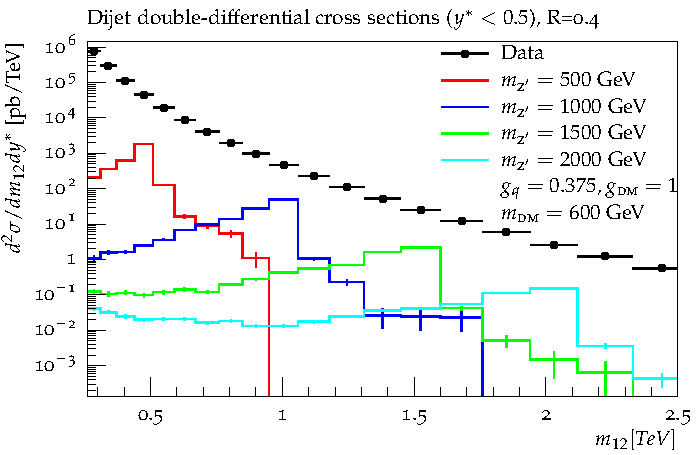
\includegraphics[width=0.45\textwidth]{images/atlasdijet/fullscale/ATLAS_dijet.pdf}
      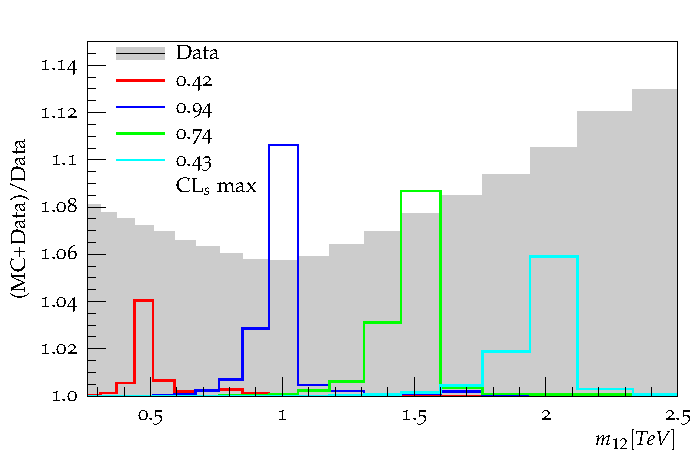
\includegraphics[width=0.45\textwidth]{images/atlasdijet/ratio/ATLAS_dijet_ratio.pdf}
    \caption{ Outputs from \rivet for a measurement included in the limit setting process. Simulated signals for a sample of mediator masses are shown, superimposed 
on the double differential inclusive jet cross section in the most central rapidity region, binned by dijet mass and rapidity as measured by ATLAS at 
7 TeV~\cite{Aad:2014pua}. The left hand plot compares the measured cross section to the model expectation, and the right hand plot shows the perturbation 
in the ration compared to the relative uncertainty in the measurement. 
The signals form a 1D parameter space scan in mediator mass for fixed dark matter mass and mediator couplings; $\MDM=600$ GeV, 
$\GQ=0.25$ and $\GDM = 1$.}
\label{fig:ATLASdijet}
\end{figure}

\todo{MK: I prefer larger figures, see below, but leave this to you to decide.}

\begin{figure}[!htb]
\centering
      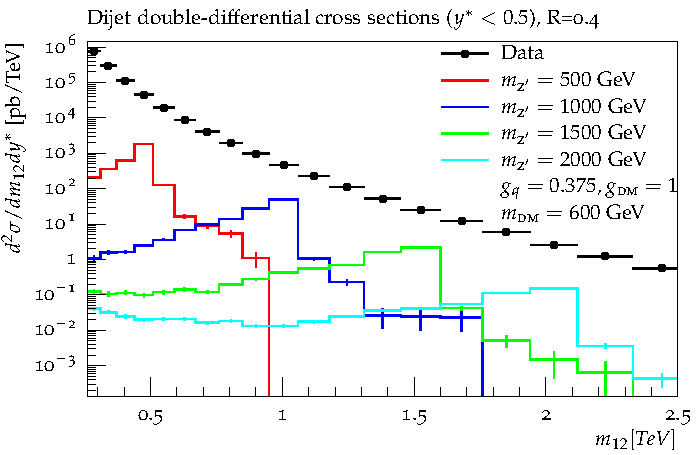
\includegraphics[width=0.9\textwidth]{images/atlasdijet/fullscale/ATLAS_dijet.pdf}\\
      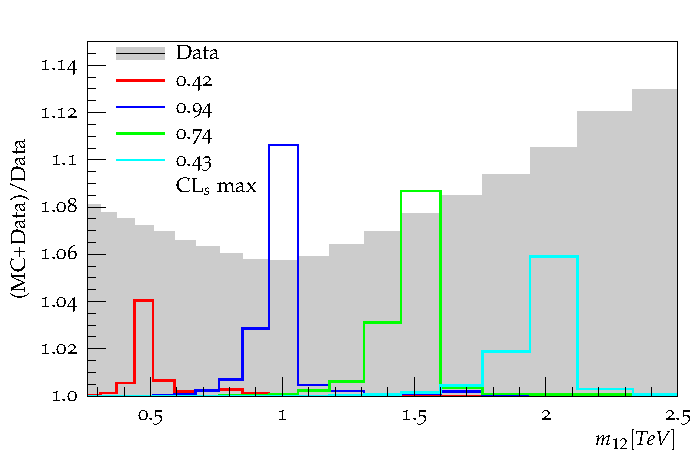
\includegraphics[width=0.9\textwidth]{images/atlasdijet/ratio/ATLAS_dijet_ratio.pdf}
    \caption{ Outputs from \rivet for a measurement included in the limit setting process. Simulated signals for a sample of mediator masses are shown, superimposed 
on the double differential inclusive jet cross section in the most central rapidity region, binned by dijet mass and rapidity as measured by ATLAS at 
7 TeV~\cite{Aad:2014pua}. The left hand plot compares the measured cross section to the model expectation, and the right hand plot shows the perturbation 
in the ration compared to the relative uncertainty in the measurement. 
The signals form a 1D parameter space scan in mediator mass for fixed dark matter mass and mediator couplings; $\MDM=600$ GeV, 
$\GQ=0.25$ and $\GDM = 1$.}
\label{fig:ATLASdijet}
\end{figure}

Figure~\ref{fig:ATLASdijet} shows a comparison between the model expectations in the `challenging' scenario and the most sensitive distributions from the ATLAS jet measurements. The measured 
dijet mass distribution is smoothly falling to higher masses, and the presence of a mediator decaying to quarks would superimpose a
peak, not seen in the data, thus leading to an exclusion. The results are shown for fixed $\MDM = 600$~GeV and a range of mediator massses $500 < \MZP < 2000$~GeV. 
The sensitivity is at maximum in the middle of this range.

\begin{figure}
\centering      
      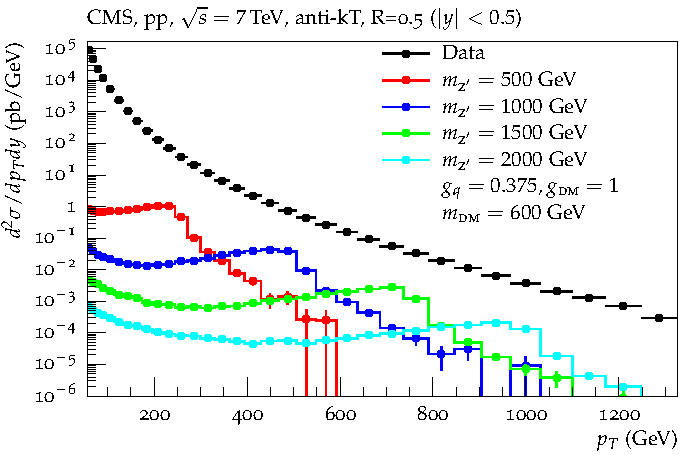
\includegraphics[width=0.45\textwidth]{images/cmsjet/fullrange/CMSincljet.pdf}
      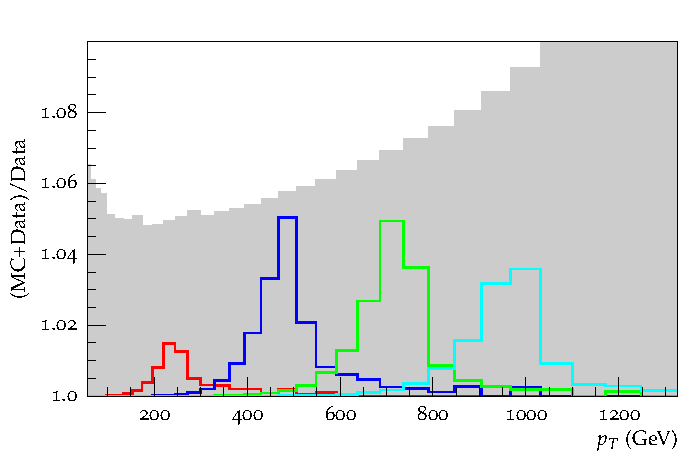
\includegraphics[width=0.45\textwidth]{images/cmsjet/ratio/CMSincljets_ratio.pdf}
\caption{Outputs from \rivet for a measurement included in the limit setting process. Simulated signals for a sample of mediator masses are shown, superimosed on 
the double differential dijet cross section in the most central rapidity region, binned by leading jet \pt and rapidity as measured by 
CMS at 7 TeV~\cite{Chatrchyan:2014gia}. The left hand plot compares the measured cross section to the model expectation, and the right hand plot shows the perturbation 
in the ration compared to the relative uncertainty in the measurement. The signals form a 1D parameter space scan in mediator mass for fixed dark matter mass 
and mediator couplings; $\MDM=600$ GeV, $\GQ=0.25$ and $\GDM = 1$.}
\label{fig:CMSincljet}
\end{figure}

Figure~\ref{fig:CMSincljet} shows a similar comparison for a comparable measurement from CMS. This time the sensitivity is in the jet \pt distribution, but the pattern
is similar, with a maximal sensitivity for mediator masses around 1~TeV. These measurements typify the sensitivies obtained from the `Jets' measurements discussed in
Section~\ref{sec:measurements}. It is notable that 7~TeV measurements form the bedrock of the exclusions. This is due to the lack of availability of precision
8~TeV and 13~TeV measurements in \rivet. Such measurements are likely to be available soon and can be expected to significantly improve the exclusion power of these
final states.

\begin{figure}
\centering
      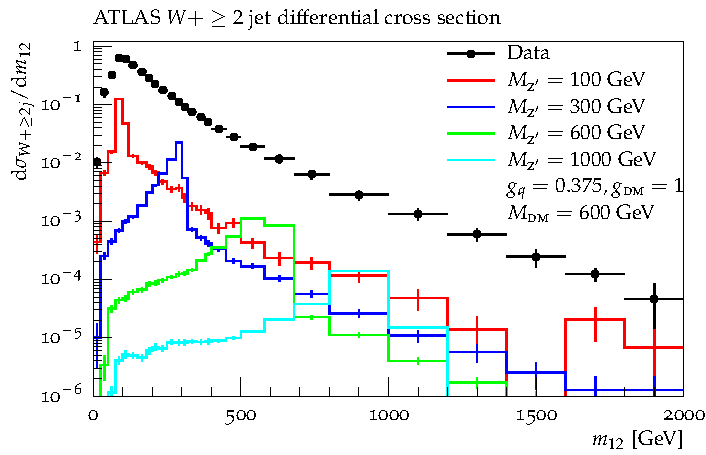
\includegraphics[width=0.45\textwidth]{images/atlaswjet/fullrange/ATLASWjet.pdf}
      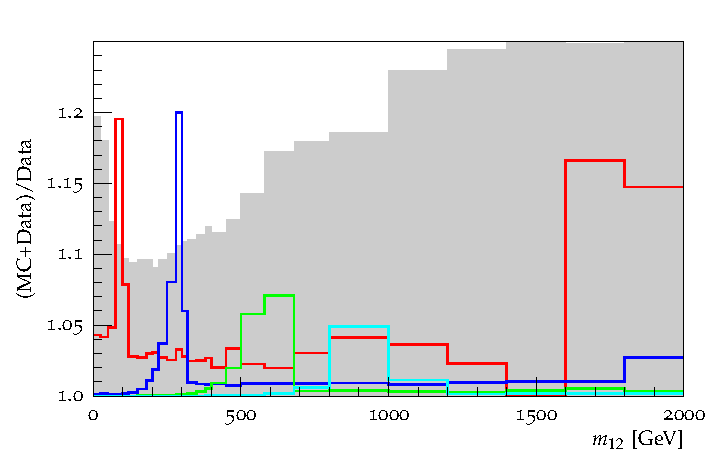
\includegraphics[width=0.45\textwidth]{images/atlaswjet/ratio/ATLASwjet_ratio.pdf}
\caption{Outputs from \rivet for a measurement included in the limit setting process. Simulated signals for a sample of mediator masses, superimposed on 
the differential cross section for the $W+\geq2$ jet process, binned in the mass of the dijet pair as measured by ATLAS at 7 TeV~\cite{Aad:2014qxa}.
The signals form a 1D parameter space scan in mediator mass for fixed dark matter mass and mediator couplings; $\MDM=600$ GeV, $\GQ=0.25$ and $\GDM = 1$.}
\label{fig:ATLASwjet}
\end{figure}

Moving on to the `electroweak' final states discussed in Section~\ref{sec:measurements}, Figure~\ref{fig:ATLASwjet} illustrates the sensitivity of vector-boson-plus-jet
($V+$jet) measurements to this model, in this case the dijet mass differential cross section in $W+$-jet events. Strictly speaking, the measurement is made for
events with a single charged lepton, \MET, and jets, interpreted as $W$+jets in the SM. In the BSM model considered here, \MET could in principle 
also arise from the dark matter candidate. However, inspections shows that the sensitivity -- which is at mediator masses below around a TeV or so -- arises 
from genuine $W$ bosons produced in association with the mediator -- not a signature typically considered in constraints on this class of model. The sensitivity
is obviously highly dependent upon the bin width chosen in the SM measurement, which is driven mainly by the dijet mass resolution, although at high masses also by
the number of events in the data.

\begin{figure}
\centering
      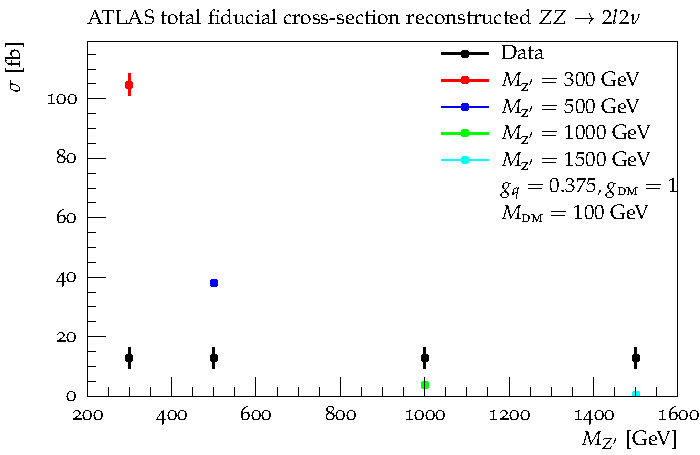
\includegraphics[width=0.45\textwidth]{images/atlaszz/fullrange/ATLASZZ.pdf}
\caption{Outputs from \rivet for a potential measurement to be included in the limit setting process. Simulated signals for a 
sample of mediator masses, interpreted as perturbations to the $ZZ\rightarrow l^+l^- \MET$ cross section 
corresponding to the data as measured by ATLAS at 7 TeV~\cite{Aad:2012awa} \label{fig:ATLASzz}. The signals form a 1D parameter space scan in 
mediator mass \MZP for fixed dark matter mass and mediator couplings; $\MDM=100$ GeV, $g_{q}=0.25$ and $g_{\textsc{dm}} = 1$.}
\label{fig:ATLASzz}
\end{figure}

Also in the `electroweak' category are the diboson measurements. Here the most sensitive is the ATLAS $ZZ$ measurement, in particular the 7~TeV result, which includes
a fiducial cross section measurement of $pp \rightarrow l^+l^- + \MET$, interpreted in the paper as $pp \rightarrow ZZ \rightarrow l^+l^- \nu \bar{\nu}$, but performed in a 
sufficiently model-independent fashion that it has the same sensitivity to the $l^+l^- +$ dark matter channel. This is illustrated in Fig.~\ref{fig:ATLASzz}.
The production diagrams are the same as the $V$-jets case, but in this case the 
mediator decays to dark matter rather than back to quarks. \todo{MK: maybe we should show a couple of example Feynman diagrams at some point?}
In the absence of any particle-level measurements in the `missing energy plus jets' category of 
Section~\ref{sec:measurements}, this measurement has the best sensitivity to dark matter production for this model. Obviously, measurements at 8~TeV and 13~TeV of this 
final state, and indeed of jets+\MET, can be expected to improve the sensitivity significantly.

Finally, although they were scanned in the limit-setting process, the currently available isolated photon measurements do not contribute signficantly to the exclusion
limits for this model.

\section{Limits}\label{sec:limits}

The sensitivities derived from multiple distributions such as those discussed in the previous section are combined into `heatmaps' which delineate exclusion 
regions and contours in the parameter space of \MDM and \MZP. These are shown in Fig.~\ref{fig:maps} for the three \GQ values considered.
Several features are discernible. 

As expected, the exclusion is much weaker in the `challenging' case and quite strong in the `optimistic' scenario.

For the first three scenarios, at $\MZP > 2\MDM$ the decay of the mediator to dark matter dominates over the decay to jets. This leads to the diagonal structure across the plots, 
with the sensitivity below the diagonal, in the right portion of the map, coming mainly from the jet measurements. In the fourth scenario, even when the decay to
DM is kinematically allowed, the jet signatures continue to contribute, and so the diagonal structure is less visible. 

At low values of the \MZP the sensitivity comes mainly from the $V+$jets signatures. In the challenging and intermediate scenarios, a dip in sensitivity around 
$\MZP \approx 700$~GeV is visible, where the sensitvity from inclusive jets and $V+$jets do not quite overlap. In the optimistic scenario, they overlap, and the whole lower
right region of the map is excluded. In addition, the cross section $\times$ branching ratio for quarks $\rightarrow Z^\prime \rightarrow$ quarks remains large
enough that the diagonal cutoff in sensitivity of the jet channels at $\MZP \approx 2\MDM$ is blurred. 

To the top left region of the diagonal the decay of the mediator to dark matter is kinematically allowed, and for $\GDM=1$ it will dominate 
over the decay to quarks. Hence the sensitivity in the inclusive jet (and $V+$jet) signatures drops in all scenarios except the fourth. 
This is the region where a measurement of \MET+jets would be useful 
(and indeed it is where the searches performed using such signatures contribute, see \cite{Kahlhoefer:2015bea}). Current sensitivity in the intermediate and challenging scenarios 
comes from the $l^+l^- + \MET$ measurement, and dies away at $\MZP \approx 750$~GeV. In the fourth scenario, the decays to dark matter are relatively suppressed and 
so the $l^+l^- + \MET$ signature makes little contribution. However, as already discussed, the exclusion from the jet measurements remains strong.


\begin{figure}[p]
\centering
\hfill
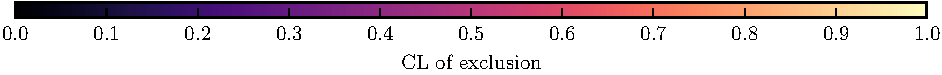
\includegraphics[width=.95\textwidth]{analysis/plots/colorbarkey.pdf}
\centering
	\subfloat[$\GQ=0.25$ and $\GDM = 1$\label{fig:map025}]{%
    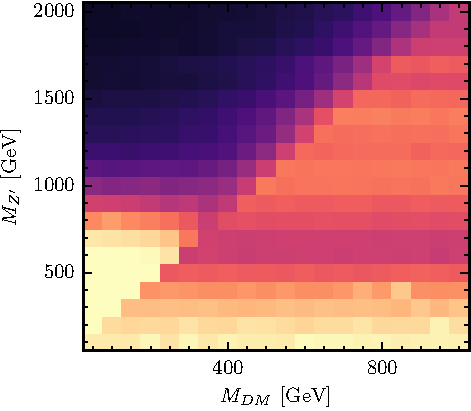
\includegraphics[width=0.5\textwidth]{analysis/plots/combinedCL_gq025.pdf}
    }
    \subfloat[$\GQ=0.5$ and $\GDM = 1$\label{fig:map05}]{%
    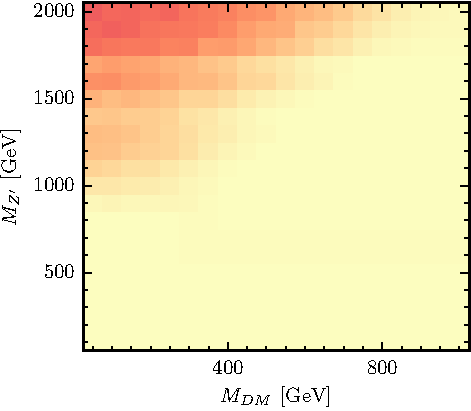
\includegraphics[width=0.5\textwidth]{analysis/plots/combinedCL_gq05.pdf}
    }
    
    \subfloat[$\GQ=0.375$ and $\GDM = 1$\label{fig:map0375}]{%
    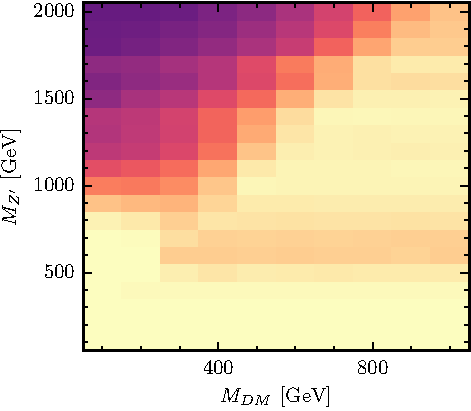
\includegraphics[width=0.5\textwidth]{analysis/plots/combinedCL_gq0375.pdf}
    }
    \subfloat[$\GQ=0.375$ and $\GDM = 0.25$\label{fig:map0375_025}]{%
    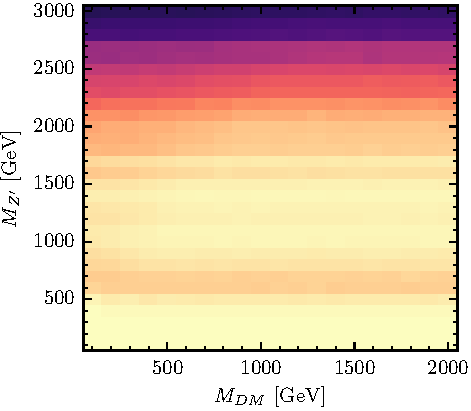
\includegraphics[width=0.5\textwidth]{analysis/plots/combinedCL_gq0375_gdm025.pdf}
    }

    \caption{Heatmaps displaying 2D parameter space scans in fixed mass planes corresponding to a fixed $g_{\textsc{dm}} = 1$ and variable $g_{q}$, with
    figure~\ref{fig:map025} representing $g_{q}=0.25$ and figure~\ref{fig:map05} representing $g_{q}=0.5$. The confidence level of exclusion represented 
    corresponds to testing the full signal strength hypothesis against the null background only hypothesis, calculated as outlined in 
    section~\ref{sec:statmethod}. The combination of measurements entering into the confidence level presented here is the maximally
    sensitive allowed grouping as outlined in section~\ref{sec:dynselec}, considering all available measurements as listed in section~\ref{sec:measurements}.
    (a) Challenging scenario, (b) Optimistic (c) Intermediate (d) DM suppressed.}

    \label{fig:maps}
\end{figure}

The 95\% contours derived from the heatmaps of Fig.~\ref{fig:maps} are shown in Fig.~\ref{fig:cont}.

\begin{figure}[p]
\centering
    \subfloat[$\GQ=0.25$ and $\GDM = 1$ \label{fig:cont025}]{%
    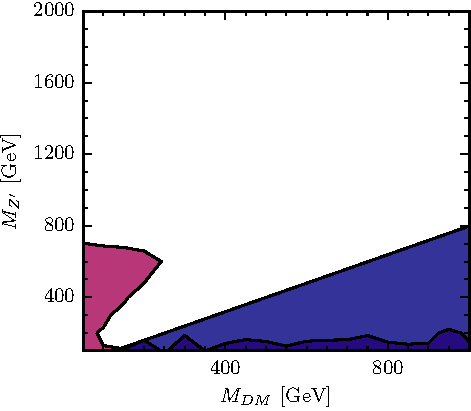
\includegraphics[width=0.5\textwidth]{analysis/plots/contour_gq025.pdf}
    }
    \subfloat[$\GQ=0.5$ and $\GDM = 1$\label{fig:cont05}]{%
      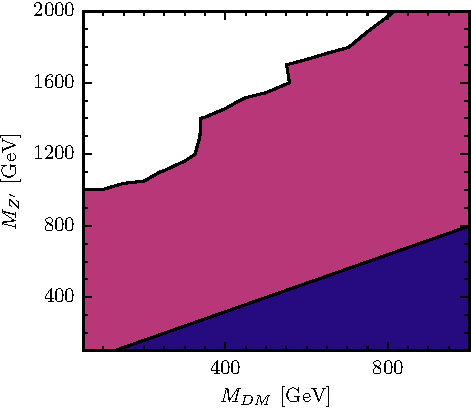
\includegraphics[width=0.5\textwidth]{analysis/plots/contour_gq05.pdf}
    }

    \subfloat[$\GQ=0.375$ and $\GDM = 1$\label{fig:cont0375}]{
      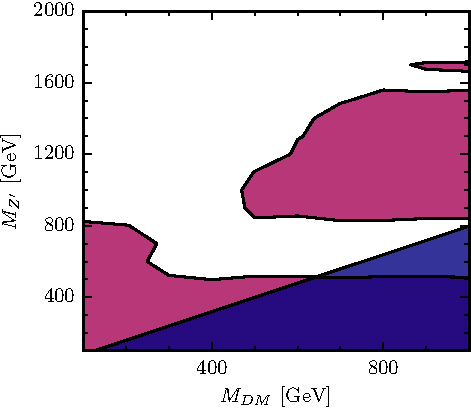
\includegraphics[width=0.5\textwidth]{analysis/plots/contour_gq0375.pdf}
    }
    \subfloat[$\GQ=0.375$ and $\GDM = 0.25$\label{fig:cont0375_025}]{%                
      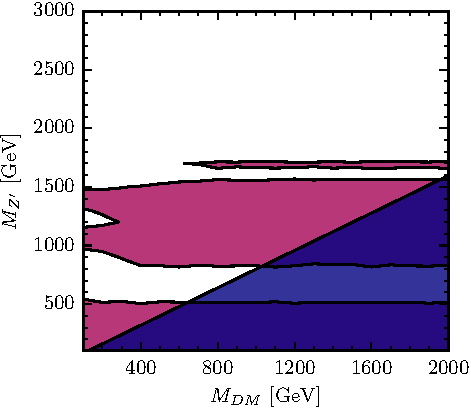
\includegraphics[width=0.5\textwidth]{analysis/plots/contour_gq0375_gdm025.pdf}
    }
\caption{Placeholder contours, 95 CL in Purple, pert unitarity excluded overlaid in blue}\label{fig:cont}
\end{figure}

As mentioned in section~\ref{sec:model},  the parameters of the simplified model are constrained by perturbative unitarity. 
In the region $\MDM \gtrsim \sqrt{\pi/2}\, \MZP/g_{\rm DM}$, indicated by the blue shaded area in Fig.~\ref{fig:cont}, 
the dark matter relic density cannot be calculated reliably~\cite{Kahlhoefer:2015bea}. Since we only consider couplings \GDM and \GQ well within the perturbative regime, perturbative unitarity is respected in the production of mediators at the LHC 
and does not provide any further restrictions on the parameter space of our model~\cite{Englert:2016joy}. The physics of dark matter is, of course, constrained by astrophysical and cosmological observations, including in particular the dark matter relic density, and direct and indirect searches for dark matter, see e.g.\ Refs.~\cite{Kahlhoefer:2015bea, Heisig:2015ira,Jacques:2016dqz} for combined analyses of collider and astrophysical constraints of simplified dark matter models with vector mediators. However, all those constraints are based on additional assumptions on the thermal history of the Universe and astrophysical properties of dark matter, and they do not affect BSM searches at the LHC. Since we have adopted the simplified dark matter model to illustrate the power of the \Contur approach for BSM searches at the LHC in general, rather than providing a detailed cosmological and astrophysical analysis of dark matter, we do not show the corresponding constraints in Fig.~\ref{fig:cont}. 


\todo{here we should have some discussion of the theory constraints, other experiment constraints, and cosmological context.}

Note that as expected, the sensitivity from the 7~TeV dijet measurements used here is qualitatively similar, but inferior, to the exclusions obtained 
combining the searches in 8~TeV and 13~TeV jet data - see, for example, \cite{Fairbairn:2016iuf}. This should change once measurements
are available from these later running periods (indeed, the CMS measurement is already made~\cite{Khachatryan:2016wdh}, but is not yet available in \rivet or HepData).
(Looks like the $ZZ$ analyis picks off a bit of phase space for $\MDM < 250$~GeV, $\MZP < 750$~GeV which isn't covered in Fig.3 or \cite{Fairbairn:2016iuf}?)


\section{Conclusions}\label{sec:conclusions}

Using a simplified model for weakly-interacting dark matter coupled to the Standard Model via a heavy mediator boson, we have developed and demonstrated 
a method to efficently scan existing particle-level measurements from the LHC, implemented in \rivet, to derive limits on new physics. 
The \Contur method uses measurements which have already been shown to be in good agreement with the SM, and thus is purely aimed at limiting the possibilities 
for models of new physics and hopefully narrowing the focus of experimental and theoretical effort on to the best models. It is thus complementary to 
direct and dedicated searches. The exclusion limits obtained are competitive with limits from searches to  date which have reported null results.
One notable feature is the simultaneous coverage of a wide variety final states. This leads to enhanced stability of the sensitivity as a function of model
parameters, and also can uncover sensitivity in channels which might not otherwise be considered. For example, in our case unexpected sensitivity is seen in
$V$+jets measurements, as well as the more commonly used dijet and \MET channels. The method is highly scaleable to new measurements as they are produced, and
to new simplified models as they are developed.

\section*{Acknowledgments}
This work started at the `Interdisciplinary Workshop on ‘Models, simulations and data at LHC' in Edinburgh, and continued in the 2015 Les Houches meeting on 
TeV-scale physics and two MCnet schools in G\"ottingen. The authors thank the organisers, especially Michela Massimi, Fawzi Boudjema and Steffen Schumann. 
They also thank Josh McFayden for useful discussions, and STFC for financial support. MK is supported by the German Research Foundation DFG through the research unit 2239 ``New physics at the LHC".

%\clearpage
\bibliographystyle{h-physrev4}
\bibliography{simple}

\end{document}


